\documentclass[aspectratio=169,10pt,t]{beamer}
%------------------------------------------------------------------
\usepackage{iftex}
\ifPDFTeX
\usepackage[scaled=0.95]{helvet}
\else
\usepackage{fontspec}
\IfFontExistsTF{Helvetica Neue}{%
    \setmainfont{Helvetica Neue}%
    \setsansfont{Helvetica Neue}%
}{%
    \setmainfont{TeX Gyre Heros}%
    \setsansfont{TeX Gyre Heros}%
}%
\fi
\renewcommand{\familydefault}{\sfdefault}
\usefonttheme{professionalfonts}

\usepackage{graphicx}
\usepackage{xurl}
\usepackage{tikz}
\usetikzlibrary{arrows.meta,calc,positioning}
\usepackage[most]{tcolorbox}
\usepackage{booktabs,array,colortbl,tabularx}
\hyphenpenalty=10000 \exhyphenpenalty=10000

%------------------------------------------------------------------
% INFO PRESENTASI (EDIT DI SINI)
%------------------------------------------------------------------
\newcommand{\teamnames}{Bastian Ramy Ervandi (Ketua) \textperiodcentered{} Muhammad Bryan Farras \textperiodcentered{} Grace Yunike Margaretha Sitorus \textperiodcentered{} Muhammad Haidar Al Ghifari \textperiodcentered{} Rafsya Ghaizan Athari}
\newcommand{\supervisor}{Yan Maraden, S.T., M.T.}
\newcommand{\presdate}{Oktober 2026}

%------------------------------------------------------------------
% PALET: putih bersih + biru dan kuning (mengikuti Evaluasi Akademik)
%------------------------------------------------------------------
\definecolor{rblue}{HTML}{0A00FF}
\definecolor{ryel}{HTML}{FFD400}
\definecolor{ink}{HTML}{111111}
\definecolor{slate}{HTML}{5F6368}
\definecolor{mist}{HTML}{F4F4F4}
\definecolor{track}{HTML}{E4E4E4}
\definecolor{rule}{HTML}{D6D6D6}
\definecolor{okgreen}{HTML}{16A34A}
\definecolor{badred}{HTML}{E11D48}

%------------------------------------------------------------------
% TEMA BEAMER
%------------------------------------------------------------------
\setbeamertemplate{navigation symbols}{}
\setbeamercolor{background canvas}{bg=white}
\setbeamercolor{normal text}{fg=ink}
\setbeamersize{text margin left=0.7cm,text margin right=0.7cm}
\setbeamertemplate{itemize item}{\raisebox{0.25ex}{\color{rblue}\tiny$\bullet$}}
\setbeamertemplate{itemize subitem}{\color{rblue}\tiny$\circ$}
\setbeamerfont{itemize/enumerate body}{size=\normalsize}
\setbeamerfont{itemize/enumerate subbody}{size=\small}
\setlength{\leftmargini}{1.1em}

% Penanda bagian: nomor (kotak kuning) + label (miring biru, kanan atas)
\gdef\currnum{00}
\gdef\currlabel{}
\newcommand{\sect}[2]{\gdef\currnum{#1}\gdef\currlabel{#2}}

% Header: kotak kuning (pengganti logo), judul tebal, garis biru, label kanan
\setbeamertemplate{frametitle}{%
    \begin{tikzpicture}[remember picture,overlay]
        \fill[ryel] (current page.north west) rectangle ++(1.3,-0.82);
        \node[text=rblue,font=\large\bfseries] at ($(current page.north west)+(0.65,-0.41)$) {\currnum};
        \node[anchor=base west,inner sep=0pt,font=\Large\bfseries,text=ink]
        at ($(current page.north west)+(2.1,-0.6)$) {\insertframetitle};
        \node[anchor=south east,inner sep=0pt,font=\footnotesize\itshape,text=rblue]
        at ($(current page.north east)+(-0.25,-0.5)$) {\currlabel};
        \draw[rblue,line width=1.1pt]
        ($(current page.north west)+(2.0,-0.82)$) -- ($(current page.north east)+(-0.2,-0.82)$);
    \end{tikzpicture}%
    \vskip 0.2cm
}

% Footer: pil abu muda di tengah bawah (seperti deck Evaluasi Akademik)
\setbeamertemplate{footline}{%
    \leavevmode\hbox to\paperwidth{%
        \rule{0pt}{0.95cm}%
        \begin{tikzpicture}[remember picture,overlay]
            \fill[mist,rounded corners=0.4cm]
            ($(current page.south)+(-5.6,-0.6)$) rectangle ($(current page.south)+(5.6,0.66)$);
            \node[anchor=west,inner sep=0pt,font=\footnotesize,text=ink]
            at ($(current page.south)+(-5.2,0.2)$)
                {Desain Proyek 2 \textperiodcentered{} Kelompok 9 \textperiodcentered{} Autonomous Rover SLAM};
            \draw[rule,line width=0.6pt] ($(current page.south)+(3.75,0.06)$) -- ($(current page.south)+(3.75,0.36)$);
            \node[font=\footnotesize\bfseries,text=rblue,inner sep=0pt]
            at ($(current page.south)+(4.7,0.2)$) {\insertframenumber\,/\,\inserttotalframenumber};
        \end{tikzpicture}\hfil}%
}

%------------------------------------------------------------------
% KOMPONEN VISUAL
%------------------------------------------------------------------
% Bilah judul biru (dan varian kuning) dengan sudut membulat
\newcommand{\lbar}[1]{%
    \begin{tcolorbox}[enhanced,colback=rblue,colframe=rblue,coltext=white,boxrule=0pt,arc=5pt,
        left=4pt,right=4pt,top=3.5pt,bottom=3.5pt,halign=center,fontupper=\bfseries,
        before skip=0pt,after skip=5pt]#1\end{tcolorbox}}
\newcommand{\lbary}[1]{%
    \begin{tcolorbox}[enhanced,colback=ryel,colframe=ryel,coltext=rblue,boxrule=0pt,arc=5pt,
        left=4pt,right=4pt,top=3.5pt,bottom=3.5pt,halign=center,fontupper=\bfseries,
        before skip=0pt,after skip=5pt]#1\end{tcolorbox}}

% Panel bergaris putus-putus biru (isi Key Takeaway dan catatan)
\newtcolorbox{dpanel}[1][]{enhanced,frame hidden,halign=flush left,colback=white,boxrule=0pt,arc=5pt,
    left=8pt,right=8pt,top=5pt,bottom=5pt,before skip=0pt,after skip=0pt,
    overlay={\draw[rblue,dash pattern=on 4pt off 3pt,line width=0.8pt,rounded corners=5pt]
    (frame.south west) rectangle (frame.north east);},#1}

% Key Takeaway: bilah biru + panel putus-putus  \takeaway[Judul]{isi}
\newcommand{\takeaway}[2][Key Takeaway]{%
    \par\vspace{5pt}%
    \begin{tcolorbox}[enhanced,colback=rblue,colframe=rblue,coltext=white,boxrule=0pt,arc=5pt,
        left=4pt,right=4pt,top=2.5pt,bottom=2.5pt,halign=center,fontupper=\bfseries\itshape,
        before skip=0pt,after skip=3pt]#1\end{tcolorbox}%
    \begin{dpanel}\small #2\end{dpanel}}

% Key Takeaway ringkas (tanpa bilah judul), untuk slide yang padat: \takeawayc{isi}
\newcommand{\takeawayc}[1]{%
    \par\vspace{6pt}\begin{dpanel}\small\textbf{\color{rblue}Key takeaway:} #1\end{dpanel}}

% Penanda istilah penting: sorot kuning (teks biru) / sorot biru (teks putih)
\newcommand{\hl}[1]{{\setlength{\fboxsep}{1.2pt}\colorbox{ryel}{\bfseries\color{rblue}#1}}}
\newcommand{\hb}[1]{{\setlength{\fboxsep}{1.2pt}\colorbox{rblue}{\bfseries\color{white}#1}}}

% Daftar bernomor dengan lingkaran: \nitem (biru) dan \nitemy (kuning)
\newcommand{\nitemgen}[4]{% isi lingkaran, teks lingkaran, nomor, teks
    \par\noindent\begin{minipage}[t]{0.095\linewidth}%
    \tikz[baseline=(c.base)]\node[circle,fill=#1,text=#2,minimum size=0.58cm,inner sep=0pt,
        font=\small\bfseries](c){#3};%
    \end{minipage}\hfill%
    \begin{minipage}[t]{0.885\linewidth}\raggedright #4\end{minipage}\par\vspace{7pt}}
\newcommand{\nitem}[2]{\nitemgen{rblue}{white}{#1}{#2}}
\newcommand{\nitemy}[2]{\nitemgen{ryel}{rblue}{#1}{#2}}

% Kartu info dengan garis aksen di kiri: \infocard[warna]{Judul}{isi}
\newcommand{\infocard}[3][rblue]{%
    \begin{tcolorbox}[enhanced,colback=white,colframe=rule,boxrule=0.6pt,arc=4pt,
        borderline west={3.5pt}{0pt}{#1},halign=flush left,left=9pt,right=7pt,top=5pt,bottom=5pt,
        before skip=0pt,after skip=6pt]
    {\bfseries\color{rblue}#2}\par\vspace{2pt}#3
    \end{tcolorbox}}

% Kartu fase dengan judul biru dan tinggi tetap: \begin{phase}{tinggi}{Judul}
\newtcolorbox{phase}[2]{enhanced,colback=white,colframe=rule,boxrule=0.6pt,arc=5pt,height=#1,
    title=#2,colbacktitle=rblue,coltitle=white,fonttitle=\bfseries,halign title=center,
    toptitle=2.5pt,bottomtitle=2.5pt,left=7pt,right=6pt,top=6pt,bottom=4pt,
    before skip=0pt,after skip=0pt}

% Label status kecil
\newcommand{\chip}[3]{\tikz[baseline=(c.base)]\node[fill=#2,text=#3,rounded corners=3pt,
    inner xsep=5pt,inner ysep=2.5pt,font=\scriptsize\bfseries](c){#1};}
\newcommand{\lulus}{\chip{LULUS}{okgreen}{white}}
\newcommand{\proses}{\chip{PROSES}{ryel}{rblue}}
\newcommand{\belum}{\chip{BELUM}{badred}{white}}
\newcommand{\teratasi}{\chip{TERATASI}{okgreen}{white}}
\newcommand{\tercapai}{\chip{TERCAPAI}{okgreen}{white}}
\newcommand{\gagal}{\chip{TIDAK LULUS}{badred}{white}}
\newcommand{\sebagian}{\chip{SEBAGIAN}{ryel}{rblue}}
\newcommand{\tinggi}{\chip{TINGGI}{badred}{white}}
\newcommand{\sedang}{\chip{SEDANG}{ryel}{rblue}}

% Bilah progres:  \pbar{persen}{label}
\newcommand{\pbar}[2]{%
    \begin{tikzpicture}
    \node[anchor=west,font=\small\bfseries,inner sep=0pt] at (0,0.5) {#2};
    \fill[track,rounded corners=3pt] (0,-0.16) rectangle (4.6,0.16);
    \pgfmathsetmacro{\pw}{4.6*#1/100}
    \fill[rblue,rounded corners=3pt] (0,-0.16) rectangle (\pw,0.16);
    \node[anchor=west,font=\normalsize\bfseries,text=rblue,inner sep=0pt] at (4.75,0) {#1\%};
    \end{tikzpicture}}

% Tabel: header biru, baris selang-seling putih / abu sangat muda
\newcolumntype{L}[1]{>{\raggedright\arraybackslash}p{#1}}
\newcolumntype{Y}{>{\raggedright\arraybackslash}X}
\newcommand{\hd}[1]{\bfseries\color{white}#1}
\newcommand{\tablestyle}{\small\setlength{\tabcolsep}{6pt}\setlength{\extrarowheight}{3pt}\arrayrulecolor{rule}}

%------------------------------------------------------------------
% FIGURE SLOT  \figslot{nama}{lebar}{tinggi}{deskripsi}
% Memakai figures/<nama>.png|jpg|jpeg|pdf bila ada, jika tidak -> kotak penanda.
%------------------------------------------------------------------
\newcommand{\figbox}[3]{{\setlength{\fboxsep}{0pt}\setlength{\fboxrule}{0.6pt}%
\fcolorbox{rule}{white}{\includegraphics[width=#2,height=#3,keepaspectratio]{#1}}}}
\newcommand{\figph}[4]{%
    \begin{tikzpicture}
    \node[draw=rblue,dash pattern=on 4pt off 3pt,thick,rounded corners=4pt,fill=rblue!4,
        minimum width=#2,minimum height=#3,align=center,
        text width=\dimexpr#2-0.4cm\relax,inner sep=2pt]
    {{\footnotesize\bfseries\color{rblue}GAMBAR}\\[1pt]
    {\footnotesize\color{ink}#4}\\[1pt]
    {\ttfamily\scriptsize\color{slate}\detokenize{#1}}};
    \end{tikzpicture}}
\newcommand{\figslot}[4]{%
    \IfFileExists{figures/#1.png}{\figbox{figures/#1.png}{#2}{#3}}{%
        \IfFileExists{figures/#1.jpg}{\figbox{figures/#1.jpg}{#2}{#3}}{%
            \IfFileExists{figures/#1.jpeg}{\figbox{figures/#1.jpeg}{#2}{#3}}{%
                \IfFileExists{figures/#1.pdf}{\figbox{figures/#1.pdf}{#2}{#3}}{%
                    \IfFileExists{#1.png}{\figbox{#1.png}{#2}{#3}}{%
                        \IfFileExists{#1.jpg}{\figbox{#1.jpg}{#2}{#3}}{%
                            \IfFileExists{#1.jpeg}{\figbox{#1.jpeg}{#2}{#3}}{%
                                \IfFileExists{#1.pdf}{\figbox{#1.pdf}{#2}{#3}}{%
                                    \IfFileExists{figures/#1-gif.png}{\figbox{figures/#1-gif.png}{#2}{#3}}{%
                                        \IfFileExists{#1-gif.png}{\figbox{#1-gif.png}{#2}{#3}}{%
                                            \figph{#1}{#2}{#3}{#4}}}}}}}}}}}}
\newcommand{\figcap}[1]{{\footnotesize\itshape\color{slate}#1}}

%------------------------------------------------------------------
% ORNAMEN COVER / PENUTUP (garis zig-zag putih, khas deck Evaluasi Akademik)
%------------------------------------------------------------------
\newcommand{\zigzag}{%
    \begin{scope}[white,line width=0.8pt,line join=round]
    \draw ($(current page.north west)+(2.69,0)$) -- ++(-0.68,-0.82) -- ++(0.17,-0.59)
    -- ++(-0.62,-0.73) -- ++(0.45,-0.77) -- ++(-2.01,-1.41);
    \draw ($(current page.north west)+(1.65,-0.82)$) -- ++(0.2,-0.5) -- ++(-0.72,-0.41)
    -- ++(0.24,-1.04) -- ++(-1.37,0.07);
    \draw ($(current page.south east)+(0,4.0)$) -- ++(-0.58,-1.41) -- ++(-1.5,0.26)
    -- ++(-0.65,-1.47) -- ++(-1.84,0.26) -- ++(-0.68,-0.96);
    \draw ($(current page.south east)+(0,1.86)$) -- ++(-1.71,0.2) -- ++(-0.86,-1.44)
    -- ++(-1.76,0.54) -- ++(-0.79,-0.57);
    \end{scope}}
\newcommand{\logoblock}{%
    \IfFileExists{figures/logo-ui.png}{%
        \node[anchor=north west,inner sep=0pt,fill=white] at (current page.north west)
            {\includegraphics[height=0.82cm]{figures/logo-ui.png}};}{%
        \fill[ryel] (current page.north west) rectangle ++(1.3,-0.82);
        \node[text=rblue,font=\large\bfseries] at ($(current page.north west)+(0.65,-0.41)$) {UI};}}

\begin{document}

%==================================================================
% 1 - COVER
%==================================================================
    {
        \setbeamercolor{background canvas}{bg=rblue}
        \setbeamertemplate{footline}{}
        \begin{frame}[plain]
            \begin{tikzpicture}[remember picture,overlay]
                \zigzag
                \logoblock
                \node[text width=14cm,align=center,inner sep=0pt] at ($(current page.center)+(0,0.55)$) {%
                        {\color{white}\bfseries\fontsize{24}{28}\selectfont Analisis Kemajuan dan\\Persiapan Presentasi Progres}\\[11pt]
                    {\setlength{\fboxsep}{5pt}\colorbox{ryel}{\color{rblue}\bfseries\fontsize{11}{13}\selectfont Autonomous Rover for Guidance Evacuation Routing via SLAM}}\\[10pt]
                    {\color{ryel}\rule{13.2cm}{1.2pt}}\\[8pt]
                    {\color{white}\itshape\small Week 7 \textperiodcentered{} Desain Proyek Teknik Elektro, Komputer, Biomedik 2 \textperiodcentered{} Kelompok 9}};
                \node[anchor=south west,text width=9.8cm,align=left,inner sep=0pt,text=white,font=\footnotesize]
                at ($(current page.south west)+(1.2,1.15)$) {\teamnames};
                \fill[mist,rounded corners=0.4cm]
                ($(current page.south)+(-6.6,-0.6)$) rectangle ($(current page.south)+(6.6,0.7)$);
                \node[font=\footnotesize,text=ink,inner sep=0pt] at ($(current page.south)+(0,0.22)$)
                    {Universitas Indonesia \textperiodcentered{} Dosen pembimbing: \supervisor{} \textperiodcentered{} \presdate};
            \end{tikzpicture}
        \end{frame}
    }

%==================================================================
% 2 - AGENDA
%==================================================================
    \sect{00}{Alur presentasi}
    \begin{frame}{Delapan bagian presentasi}
        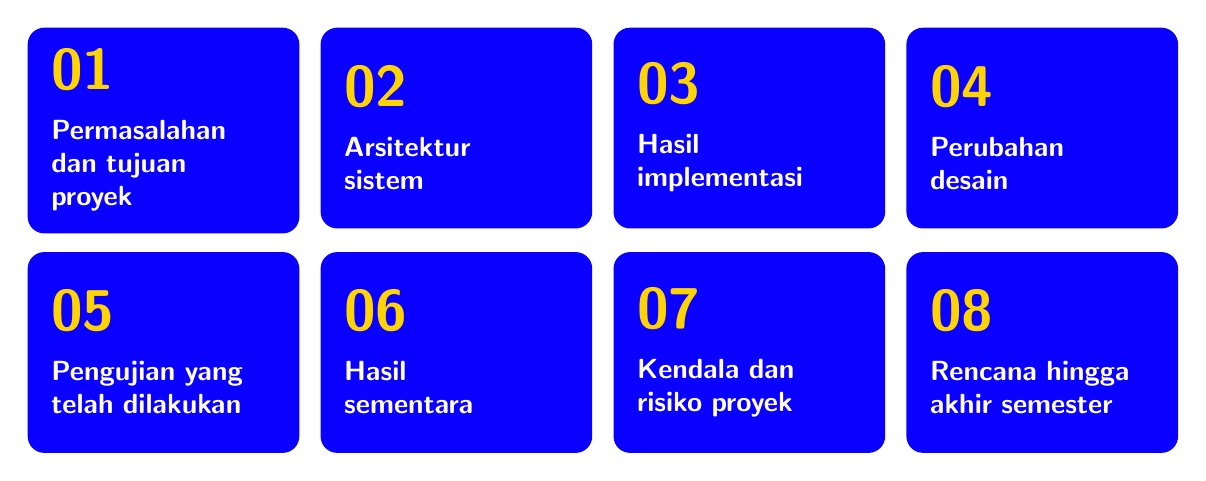
\begin{tikzpicture}
            \foreach \i/\lbl in {1/{Permasalahan\\dan tujuan proyek},2/{Arsitektur\\sistem},
            3/{Hasil\\implementasi},4/{Perubahan\\desain},5/{Pengujian yang\\telah dilakukan},
            6/{Hasil\\sementara},7/{Kendala dan\\risiko proyek},8/{Rencana hingga\\akhir semester}}{
                \pgfmathtruncatemacro{\r}{int((\i-1)/4)}
                \pgfmathtruncatemacro{\c}{mod(\i-1,4)}
                \node[anchor=north west,fill=rblue,rounded corners=6pt,
                    minimum width=3.45cm,minimum height=2.55cm,inner sep=8pt,align=left,
                    text width=2.85cm,text=white]
                at (\c*3.72,-\r*2.85) {{\fontsize{22}{24}\selectfont\bfseries\color{ryel}0\i}\\[6pt]{\bfseries\lbl}};
            }
        \end{tikzpicture}

        \vspace{6pt}
        {\footnotesize\itshape\color{slate}Dasar data: laporan kemajuan pekanan Pekan 2--7, Desain Proyek 2, Kelompok 9.}
    \end{frame}

%==================================================================
% 3 - PERMASALAHAN DAN TUJUAN
%==================================================================
    \sect{01}{Permasalahan \& tujuan proyek}
    \begin{frame}{Robot yang memandu rute evakuasi}
        \begin{columns}[T]
            \begin{column}{0.475\textwidth}
                \lbar{Permasalahan}
                \nitemy{1}{Rute evakuasi dalam gedung harus dipandu akurat, terutama bila peta belum tersedia.}
                \nitemy{2}{Robot perlu tahu posisinya sambil membangun peta (SLAM).}
                \nitemy{3}{Operator butuh pantauan telemetri dan peta secara langsung.}
            \end{column}
            \begin{column}{0.495\textwidth}
                \lbar{Tujuan Proyek}
                \nitem{1}{Memetakan dan melokalisasi robot dengan LiDAR (SLAM).}
                \nitem{2}{Bergerak otonom menghindari rintangan menuju titik evakuasi.}
                \nitem{3}{Menampilkan telemetri dan peta langsung di dashboard web.}
                \nitem{4}{Mengenali lingkungan dan objek dengan computer vision.}
            \end{column}
        \end{columns}
    \end{frame}

%==================================================================
% [BARU] TARGET KINERJA SISTEM DAN PENCAPAIANNYA
%==================================================================
    \sect{01}{Permasalahan \& tujuan proyek}
    \begin{frame}{Target kinerja sistem dan pencapaiannya}
        \tablestyle
        \renewcommand{\arraystretch}{1.0}
        % CATATAN: bila proposal memuat angka target (akurasi, latensi, dll.), tambahkan di kolom Target kinerja.
        \begin{tabularx}{\textwidth}{L{3.0cm} Y Y L{2.0cm}}
    \rowcolor{rblue}\hd{Subsistem}&\hd{Target kinerja}&\hd{Capaian saat ini}&\hd{Status}\\
    \rowcolor{white}\textbf{\color{rblue}SLAM dan lokalisasi}&Memetakan dan melokalisasi robot dengan LiDAR&Berjalan di Gazebo; masih ada drift&\proses\\
    \rowcolor{mist}\textbf{\color{rblue}Navigasi otonom}&Menghindari rintangan menuju titik evakuasi&Sistem navigasi masih dikembangkan&\proses\\
    \rowcolor{white}\textbf{\color{rblue}Monitoring}&Telemetri dan peta tampil langsung di dashboard web&UI selesai dan tampil di LCD Raspi; data ROS 2 belum terhubung&\proses\\
    \rowcolor{mist}\textbf{\color{rblue}Computer vision}&Mengenali lingkungan dan objek&Dataset dan script training siap; model belum dilatih&\proses\\
    \rowcolor{white}\textbf{\color{rblue}Hardware dan mekanik}&Rover berfungsi: chassis, PCB, dan driver motor&Chassis terakit; 3 pin driver pada PCB vendor ter-short&\proses\\
    \hline
        \end{tabularx}
        \takeawayc{Seluruh subsistem sudah berjalan sebagian; integrasi antar subsistem masih \hl{0\%}.}
    \end{frame}

%==================================================================
% 4 - ARSITEKTUR SISTEM (DIAGRAM)
%==================================================================
    \newcommand{\blk}[5]{% x, warna header, warna teks header, judul, isi
        \filldraw[fill=white,draw=rule,rounded corners=5pt] (#1,0) rectangle ++(3.4,-3.9);
        \fill[#2,rounded corners=5pt] (#1,0) rectangle ++(3.4,-0.75);
        \fill[#2] (#1,-0.4) rectangle ++(3.4,-0.35);
        \node[text=#3,font=\bfseries,inner sep=0pt] at (#1+1.7,-0.375) {#4};
        \node[anchor=north west,text width=3.0cm,align=left,font=\small,inner sep=0pt]
        at (#1+0.22,-0.98) {#5};}

    \sect{02}{Arsitektur sistem}
    \begin{frame}{Empat blok sistem, satu aliran data}
        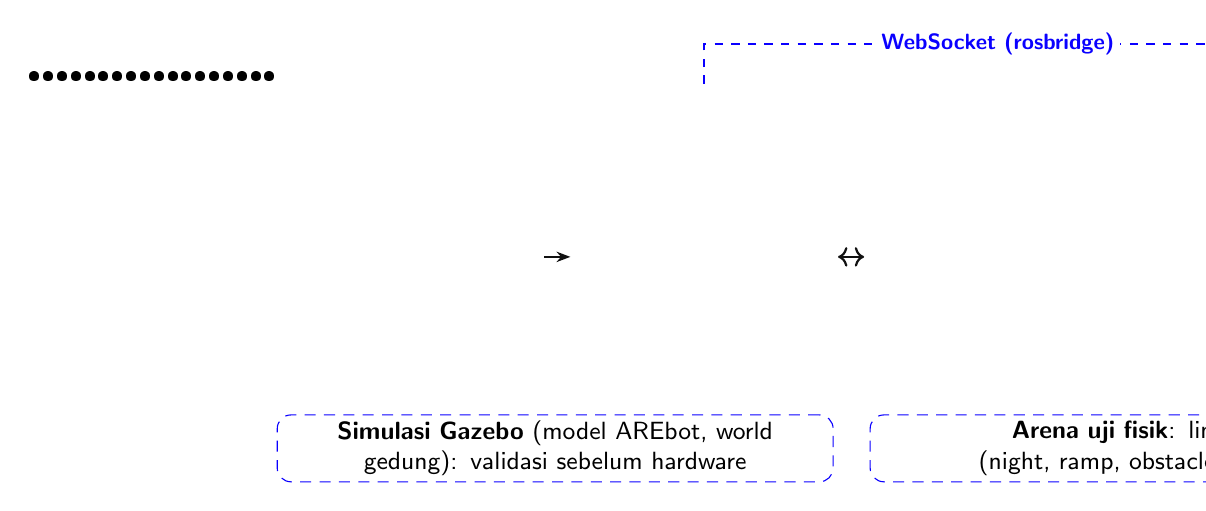
\begin{tikzpicture}[arr/.style={-{Stealth[length=5pt]},thick,ink}]
            \blk{0}{rblue}{white}{Persepsi}{\textbullet~LiDAR\\\textbullet~Raspi Camera\\\textbullet~Sensor MPU (IMU)}
            \blk{3.73}{ryel}{rblue}{Komputasi}{\textbf{Raspberry Pi 4B}\\\textbullet~ROS 2\\\textbullet~SLAM\\\textbullet~Lokalisasi\\\textbullet~Navigasi\\\textbullet~Computer vision\\\textbullet~rosbridge server}
            \blk{7.46}{rblue}{white}{Kontrol \& daya}{\textbf{PCB kustom}\\\textbullet~ESP32\\\textbullet~Manajemen daya\\\textbullet~Driver motor\\\textbullet~DC motor}
            \blk{11.19}{ryel}{rblue}{Monitoring}{\textbf{Web dashboard}\\\textbullet~Camera Feed\\\textbullet~Control: Movement dan Mode \\\textbullet~Commands\\\textbullet~System Logs\\\textbullet~Robot Status}
            \draw[arr] (3.4,-2.2) -- (3.73,-2.2);
            \draw[arr,<->] (7.13,-2.2) -- (7.46,-2.2);
            \draw[arr,dashed,rblue] (5.43,0) |- (9.16,0.5) -| (12.89,0);
            \node[font=\footnotesize\bfseries,text=rblue,fill=white,inner sep=2pt] at (9.16,0.5) {WebSocket (rosbridge)};
            \node[draw=rblue,dash pattern=on 4pt off 3pt,rounded corners=5pt,minimum width=7.06cm,minimum height=0.85cm,
                text width=6.7cm,align=center,font=\small,inner sep=2pt,anchor=north west] at (0,-4.2)
                {\textbf{Simulasi Gazebo} (model AREbot, world gedung): validasi sebelum hardware};
            \node[draw=rblue,dash pattern=on 4pt off 3pt,rounded corners=5pt,minimum width=7.06cm,minimum height=0.85cm,
                text width=6.7cm,align=center,font=\small,inner sep=2pt,anchor=north west] at (7.53,-4.2)
                {\textbf{Arena uji fisik}: limit-test (night, ramp, obstacle) + maze};
        \end{tikzpicture}
    \end{frame}

%==================================================================
% 5 - ARSITEKTUR ROVER (BLOK DIAGRAM)
%==================================================================
    \sect{02}{Arsitektur sistem}
    \begin{frame}[shrink=8]{Arsitektur ROS2 rover: sensor, proses, aktuator}
        \centering
        \scalebox{0.9}{%
        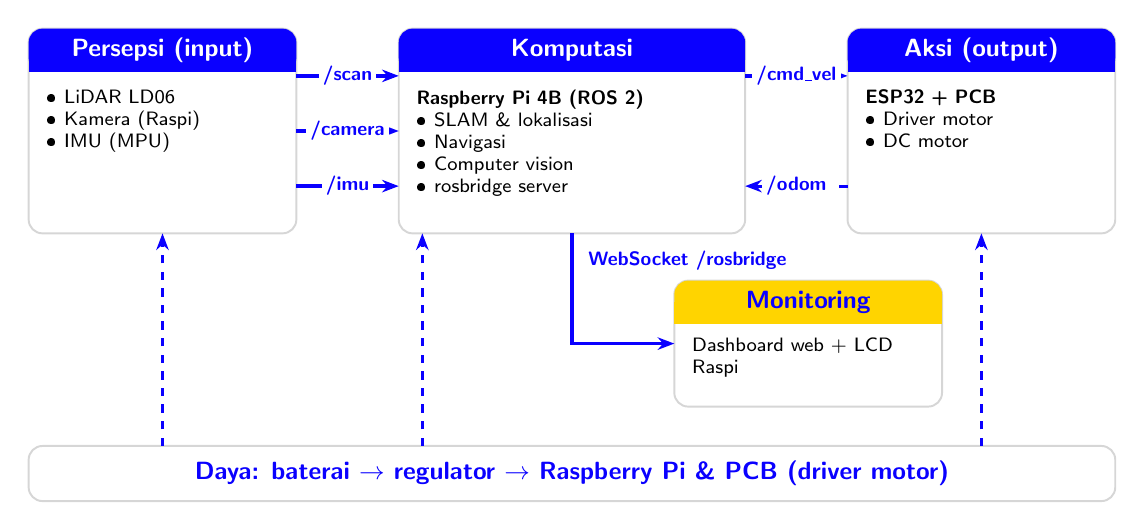
\begin{tikzpicture}[
            arr/.style={-{Stealth[length=6pt]},line width=1.2pt,rblue},
            darr/.style={-{Stealth[length=6pt]},line width=1.0pt,rblue,dashed},
            blk/.style={draw=rule,line width=0.7pt,rounded corners=5pt,fill=white},
            lbl/.style={font=\scriptsize\bfseries,text=rblue,fill=white,inner sep=1.5pt}
        ]
        % ---- Baris 1: input / proses / aktuator ----
        \filldraw[blk] (0,5.2) rectangle ++(3.4,-2.6);
        \fill[rblue,rounded corners=5pt] (0,5.2) rectangle ++(3.4,-0.55);
        \fill[rblue] (0,4.93) rectangle ++(3.4,-0.28);
        \node[text=white,font=\small\bfseries] at (1.7,4.93) {Persepsi (input)};
        \node[align=left,font=\scriptsize,inner sep=2pt,anchor=north west,text width=3.0cm] at (0.15,4.5)
            {\textbullet~LiDAR LD06\\\textbullet~Kamera (Raspi)\\\textbullet~IMU (MPU)};

        \filldraw[blk] (4.7,5.2) rectangle ++(4.4,-2.6);
        \fill[rblue,rounded corners=5pt] (4.7,5.2) rectangle ++(4.4,-0.55);
        \fill[rblue] (4.7,4.93) rectangle ++(4.4,-0.28);
        \node[text=white,font=\small\bfseries] at (6.9,4.93) {Komputasi};
        \node[align=left,font=\scriptsize,inner sep=2pt,anchor=north west,text width=4.0cm] at (4.85,4.5)
            {\textbf{Raspberry Pi 4B (ROS 2)}\\\textbullet~SLAM \& lokalisasi\\\textbullet~Navigasi\\\textbullet~Computer vision\\\textbullet~rosbridge server};

        \filldraw[blk] (10.4,5.2) rectangle ++(3.4,-2.6);
        \fill[rblue,rounded corners=5pt] (10.4,5.2) rectangle ++(3.4,-0.55);
        \fill[rblue] (10.4,4.93) rectangle ++(3.4,-0.28);
        \node[text=white,font=\small\bfseries] at (12.1,4.93) {Aksi (output)};
        \node[align=left,font=\scriptsize,inner sep=2pt,anchor=north west,text width=3.0cm] at (10.55,4.5)
            {\textbf{ESP32 + PCB}\\\textbullet~Driver motor\\\textbullet~DC motor};

        % ---- Baris 2: monitoring ----
        \filldraw[blk] (8.2,2.0) rectangle ++(3.4,-1.6);
        \fill[ryel,rounded corners=5pt] (8.2,2.0) rectangle ++(3.4,-0.55);
        \fill[ryel] (8.2,1.73) rectangle ++(3.4,-0.28);
        \node[text=rblue,font=\small\bfseries] at (9.9,1.73) {Monitoring};
        \node[align=left,font=\scriptsize,inner sep=2pt,anchor=north west,text width=3.0cm] at (8.35,1.35)
            {Dashboard web + LCD Raspi};

        % ---- Baris 3: daya ----
        \filldraw[blk] (0,-0.1) rectangle ++(13.8,-0.7);
        \node[font=\small\bfseries,text=rblue] at (6.9,-0.45)
            {Daya: baterai $\rightarrow$ regulator $\rightarrow$ Raspberry Pi \& PCB (driver motor)};

        % ---- Panah: sensor -> Raspberry Pi ----
        \draw[arr] (3.4,4.6) -- (4.7,4.6) node[midway,lbl]{/scan};
        \draw[arr] (3.4,3.9) -- (4.7,3.9) node[midway,lbl]{/camera};
        \draw[arr] (3.4,3.2) -- (4.7,3.2) node[midway,lbl]{/imu};
        % ---- Raspberry Pi <-> ESP32 ----
        \draw[arr] (9.1,4.6) -- (10.4,4.6) node[midway,lbl]{/cmd\_vel};
        \draw[darr] (10.4,3.2) -- (9.1,3.2) node[midway,lbl]{/odom};
        % ---- Raspberry Pi -> dashboard ----
        \draw[arr] (6.9,2.6) |- (8.2,1.2);
        \node[lbl,anchor=west] at (7.05,2.25) {WebSocket /rosbridge};
        % ---- Daya -> blok ----
        \draw[darr] (1.7,-0.1) -- (1.7,2.6);
        \draw[darr] (5.0,-0.1) -- (5.0,2.6);
        \draw[darr] (12.1,-0.1) -- (12.1,2.6);
        \end{tikzpicture}}

        \vspace{3pt}
        {\footnotesize\color{ink}\textbf{Persepsi} \lulus\quad \textbf{Komputasi} \proses\quad \textbf{Aksi} \sebagian\quad \textbf{Monitoring} \sebagian\quad \textbf{Integrasi} \belum}\\[4pt]
        {\footnotesize\itshape\color{slate}Sensor $\rightarrow$ Raspberry Pi memproses data untuk SLAM, navigasi, dan CV; perintah gerak dikirim ke ESP32, data dan peta dikirim ke dashboard.}
        \takeawayc{Integrasi antar subsistem masih \hl{0\%}; uji aliran data end-to-end menunggu hardware.}
    \end{frame}

%==================================================================
% [BARU] LIDAR TO MAP
%==================================================================
    \sect{02}{Arsitektur sistem}
    \begin{frame}[shrink=12]{LiDAR to map}
        \begin{columns}[T]
            \begin{column}{0.52\textwidth}
                \lbar{Dari pemindaian ke peta}
                \nitemy{1}{LiDAR memindai ruangan; data mentah masuk ke topik \texttt{/scan}.}
                \nitemy{2}{\texttt{slam\_toolbox} menyusun \hl{occupancy grid}, lalu disimpan menjadi \texttt{building\_map\_save.pgm} + \texttt{.yaml}.}
                \nitemy{3}{\texttt{nav2\_map\_server} mengirim peta ke Nav2; \hl{AMCL} memakai peta itu untuk lokalisasi robot.}
                \takeawayc{Perapian manual (bersihkan noise, pertegas dinding) membuat lokalisasi AMCL dan costmap Nav2 lebih akurat.}
            \end{column}
            \begin{column}{0.46\textwidth}
                \centering
                \begin{minipage}[t]{3.05cm}\centering
                    \figslot{fig-map-raw}{3.0cm}{4.3cm}{Peta mentah dari LiDAR}\\[2pt]\figcap{Mentah (dari LiDAR)}
                \end{minipage}\hfill
                \begin{minipage}[t]{3.05cm}\centering
                    \figslot{fig-map-polished}{3.0cm}{4.3cm}{Peta hasil polish manual}\\[2pt]\figcap{Dirapikan manual}
                \end{minipage}
            \end{column}
        \end{columns}
    \end{frame}

%==================================================================
% 6 - HASIL IMPLEMENTASI: HARDWARE
%==================================================================
    \sect{03}{Hasil implementasi}
    \begin{frame}{Hardware: komponen, PCB, dan chassis}
        \begin{columns}[T]
            \begin{column}{0.43\textwidth}
                \lbar{Hardware}
                \begin{itemize}\setlength{\itemsep}{5pt}
                    \item Komponen tersedia: LiDAR, Raspi 4B + Cam, ESP32, MPU, DC motor, LCD.
                    \item PCB vendor diterima dan disolder, tetapi 3 pin driver ter-short (bridging).
                    \item Chassis 3D print dirakit sementara; motor sudah terpasang.
                \end{itemize}
                \vspace{8pt}
                \pbar{70}{Progres hardware Pekan 7}
            \end{column}
            \begin{column}{0.55\textwidth}
                \centering
                \begin{minipage}[t]{3.9cm}\centering
                    \figslot{fig-pcb-kicad}{3.8cm}{2.4cm}{Layout dan 3D model PCB (KiCad)}\\[2pt]\figcap{Desain PCB}
                \end{minipage}\hfill
                \begin{minipage}[t]{3.9cm}\centering
                    \figslot{fig-pcb-solder}{3.8cm}{2.4cm}{PCB yang sudah disolder}\\[2pt]\figcap{PCB hasil solder}
                \end{minipage}\\[7pt]
                \begin{minipage}[t]{3.9cm}\centering
                    \figslot{fig-chassis-print}{3.8cm}{2.4cm}{Hasil 3D print chassis}\\[2pt]\figcap{Chassis hasil print}
                \end{minipage}\hfill
                \begin{minipage}[t]{3.9cm}\centering
                    \figslot{fig-chassis-assembly}{3.8cm}{2.4cm}{Assembly chassis sementara}\\[2pt]\figcap{Assembly sementara}
                \end{minipage}
            \end{column}
        \end{columns}
    \end{frame}

%==================================================================
% [BARU] PROGRESS IMPLEMENTASI ROVER (ESP32 - DRIVER - MOTOR/ENCODER)
%==================================================================
    \sect{03}{Hasil implementasi}
    \begin{frame}[shrink=5]{Progress implementasi rover}
        \begin{columns}[T]
            \begin{column}{0.44\textwidth}
                \lbar{Uji komunikasi dan encoder}
                \begin{itemize}\setlength{\itemsep}{5pt}
                    \item Rantai: \textbf{ESP32} $\rightarrow$ \textbf{driver} $\rightarrow$ \textbf{DC motor} (dengan \textbf{encoder}).
                    \item ESP32 mengirim perintah \textbf{PWM + arah}; motor bergerak.
                    \item \textbf{Pulsa encoder terbaca balik} ke ESP32 (log Serial Arduino IDE).
                    \item Baru \hl{testing awal}; sebagian jalur sudah berfungsi.
                \end{itemize}
                \vspace{4pt}
                \sebagian\ \proses
            \end{column}
            \begin{column}{0.54\textwidth}
                \centering
                \figslot{fig-arduinoIDE-encoder-log}{6.2cm}{2.9cm}{Log serial encoder di Arduino IDE}\\[2pt]\figcap{Log encoder (Arduino IDE)}\\[6pt]
                \figslot{fig-testing-lab-tekken}{6.2cm}{3.0cm}{Pengujian rangkaian di lab}\\[2pt]\figcap{Pengujian di lab}
            \end{column}
        \end{columns}
        \takeawayc{Komunikasi dasar ESP32 $\rightarrow$ driver $\rightarrow$ motor + encoder sudah terbukti; berikutnya perbaikan driver PCB dan kalibrasi encoder.}
    \end{frame}

%==================================================================
% 7 - HASIL IMPLEMENTASI: SOFTWARE
%==================================================================
    \sect{03}{Hasil implementasi}
    \begin{frame}{Software: simulasi dan dashboard}
        \begin{columns}[T]
            \begin{column}{0.485\textwidth}
                \lbar{Simulasi gedung di Gazebo}
                \centering
                \figslot{fig-gazebo-building}{6.9cm}{1.8cm}{Simulasi 3D gedung di Gazebo}
                \begin{flushleft}
                    \begin{itemize}\setlength{\itemsep}{3pt}
                        \item Mapping dan lokalisasi dasar berjalan di Gazebo.
                        \item Peta gedung tersimpan (building\_map\_save).
                        \item Body robot di simulasi diperbaiki agar LiDAR membaca posisi robot lebih akurat.
                        \item Drift lokalisasi masih diperbaiki.
                    \end{itemize}
                \end{flushleft}
            \end{column}
            \begin{column}{0.485\textwidth}
                \lbar{UI dashboard monitoring}
                \centering
                \figslot{fig-dashboard-ui}{6.9cm}{1.8cm}{Screenshot UI dashboard monitoring}
                \begin{flushleft}
                    \begin{itemize}\setlength{\itemsep}{3pt}
                        \item Lima menu: Camera Feed, Control: Movement dan Mode (Standby, Patrol, Evacuation, Manual), Robot Status, System Logs, Commands.
                        \item rosbridge\_server (WebSocket) dirombak agar stabil.
                        \item Berikutnya: logic frontend untuk data ROS 2.
                    \end{itemize}
                \end{flushleft}
            \end{column}
        \end{columns}
    \end{frame}

%==================================================================
% [BARU] PROGRESS SIMULASI SAAT INI
%==================================================================
    \sect{03}{Hasil implementasi}
    \begin{frame}[shrink=8]{progress simulasi saat ini}
        \begin{columns}[T]
            \begin{column}{0.60\textwidth}
                \centering
                \figslot{fig-sim-poster}{8.6cm}{4.8cm}{Simulasi navigasi di Gazebo dan RViz}\\[3pt]
                {\footnotesize\itshape\color{slate}Gazebo (kiri) vs RViz (kanan): robot bergerak, peta dan jalur tampil.\\[3pt]
                 \href{https://drive.google.com/file/d/1m5NwNalxrMOQDbuj7nvXKvssbHp98UR_/view?usp=sharing}{Video (Drive)}\\[2pt]
                }
            \end{column}
            \begin{column}{0.38\textwidth}
                \lbar{Simulasi navigasi}
                \begin{itemize}\setlength{\itemsep}{5pt}
                    \item World \textbf{gedung} (\texttt{building\_floor.world}).
                    \item \textbf{Gazebo}: fisika dan sensor; \textbf{RViz}: peta, costmap, pose, dan jalur.
                    \item \hl{Navigasi Nav2 sudah berjalan}: goal $\rightarrow$ jalur $\rightarrow$ robot mengikuti jalur.
                \end{itemize}
                \takeawayc{Arah dan jalur terbentuk otomatis; berikutnya memindahkan ini ke robot nyata.}
            \end{column}
        \end{columns}
    \end{frame}

%==================================================================
% 8 - [W7] HASIL IMPLEMENTASI: APP MONITORING DI LCD RASPI
%==================================================================
    \sect{03}{Hasil implementasi}
    \begin{frame}{Aplikasi monitoring pada LCD Raspi}
        \centering
        \begin{minipage}[t]{3.5cm}\centering
            \figslot{fig-app-camera}{3.4cm}{2.3cm}{Layar Camera Feed}\\[2pt]\figcap{Camera Feed}
        \end{minipage}\hfill
        \begin{minipage}[t]{3.5cm}\centering
            \figslot{fig-app-control}{3.4cm}{2.3cm}{Layar Control}\\[2pt]\figcap{Control}
        \end{minipage}\hfill
        \begin{minipage}[t]{3.5cm}\centering
            \figslot{fig-app-commands}{3.4cm}{2.3cm}{Layar Commands}\\[2pt]\figcap{Commands}
        \end{minipage}\hfill
        \begin{minipage}[t]{3.5cm}\centering
            \figslot{fig-app-logs}{3.4cm}{2.3cm}{Layar System Log}\\[2pt]\figcap{System Log}
        \end{minipage}\\[8pt]
        \begin{dpanel}
            \begin{itemize}\setlength{\itemsep}{3pt}
                \item App monitoring dirancang agar tampil di LCD yang terhubung ke Raspi.
                \item Control: Start, Pause, mode (Standby, Patrol, Evacuation, Manual), dan Emergency Stop.
                \item Commands: cek ROS nodes, system health, topik aktif, suhu CPU, status kamera, dan lainnya.
                \item Berikutnya: logic frontend untuk menerima dan memproses data simulasi ROS 2.
            \end{itemize}
        \end{dpanel}
    \end{frame}

%==================================================================
% 9 - [W7] HASIL IMPLEMENTASI: COMPUTER VISION
%==================================================================
    \sect{03}{Hasil implementasi}
    \begin{frame}{Computer vision: dataset dan script training}
        \begin{columns}[T]
            \begin{column}{0.38\textwidth}
                \centering
                \figslot{fig-cv-dataset}{5.3cm}{5.0cm}{Screenshot struktur folder Computer Vision dan Dataset CV}\\[3pt]
                \figcap{Struktur folder CV dan dataset}
            \end{column}
            \begin{column}{0.59\textwidth}
                \infocard[rblue]{Dataset}{Dataset Obstacle\_detection dengan pembagian train, valid, dan test beserta data.yaml.}
                \infocard[ryel]{Arsitektur dan script}{Arsitektur dasar model dirancang; script train\_rover.py, run\_picam\_rover.py, dan standalone\_cv.py.}
                \infocard[rblue]{Status}{Dataset dan script training 100\%; training model diundur ke Pekan 8 (model belum siap).}
            \end{column}
        \end{columns}
    \end{frame}

%==================================================================
% 10 - HASIL IMPLEMENTASI: ARENA DAN SENSOR
%==================================================================
    \sect{03}{Hasil implementasi}
    \begin{frame}{Arena uji dan sensor LiDAR}
        \centering
        \begin{minipage}[t]{4.6cm}\centering
        \end{minipage}\hfill
        \begin{minipage}[t]{4.6cm}\centering
            \figslot{fig-arena-limit}{4.5cm}{2.5cm}{Arena limit testing}\\[2pt]\figcap{Arena limit testing}
        \end{minipage}\hfill
        \begin{minipage}[t]{4.6cm}\centering
            \figslot{fig-arena-ramp}{4.5cm}{2.5cm}{Ramp testing}\\[2pt]\figcap{Uji ramp}
        \end{minipage}\\[6pt]
        \begin{minipage}[t]{4.6cm}\centering
            \figslot{fig-arena-night}{4.5cm}{2.5cm}{Arena beratap (night testing)}\\[2pt]\figcap{Arena beratap (night test)}
        \end{minipage}\hfill
        \begin{minipage}[t]{4.6cm}\centering
            \figslot{fig-lidar-test}{4.5cm}{2.5cm}{Pengujian LiDAR terbaca di laptop}\\[2pt]\figcap{LiDAR terbaca di laptop}
        \end{minipage}\hfill
        \begin{minipage}[t]{4.6cm}
            \begin{dpanel}[height=2.5cm,valign=center]
            {\bfseries\color{rblue}Status arena}\par\vspace{2pt}
                \footnotesize Limit-test sudah jadi (night, ramp, obstacle); versi maze belum jadi (dua anggota sakit, fokus pekan ini prototype) dan diundur ke Pekan 8.
            \end{dpanel}
        \end{minipage}
    \end{frame}

%==================================================================
% [BARU] KEMAMPUAN SISTEM YANG SUDAH TEREALISASI
%==================================================================
    \sect{03}{Hasil implementasi}
    \begin{frame}{Kemampuan sistem yang sudah terealisasi}
        \tablestyle
        \renewcommand{\arraystretch}{1.1}
        \begin{tabularx}{\textwidth}{L{3.6cm} Y L{2.2cm}}
    \rowcolor{rblue}\hd{Fungsi utama}&\hd{Kondisi saat ini}&\hd{Status}\\
    \rowcolor{white}\textbf{\color{rblue}Pemetaan dan lokalisasi (SLAM)}&Berjalan di Gazebo, peta gedung tersimpan, LiDAR terbaca; masih ada drift&\sebagian\\
    \rowcolor{mist}\textbf{\color{rblue}Antarmuka monitoring}&UI lima menu tampil di LCD Raspi (Camera Feed, Control, Commands, System Log); data ROS 2 belum terhubung&\sebagian\\
    \rowcolor{white}\textbf{\color{rblue}Mekanik robot}&Chassis 3D print terakit sementara; motor terpasang&\sebagian\\
    \rowcolor{mist}\textbf{\color{rblue}Kontrol daya dan driver motor}&PCB vendor disolder, 3 pin driver ter-short; driver sementara di breadboard&\belum\\
    \rowcolor{white}\textbf{\color{rblue}Computer vision}&Dataset dan script training siap; model belum dilatih&\sebagian\\
    \rowcolor{mist}\textbf{\color{rblue}Integrasi antar subsistem}&Belum diimplementasikan (0\%)&\belum\\
    \hline
        \end{tabularx}
    \end{frame}

%==================================================================
% 11 - PERUBAHAN DESAIN
%==================================================================
    \sect{04}{Perubahan desain}
    \begin{frame}{Perubahan desain: awal vs sekarang}
        \tablestyle
        \renewcommand{\arraystretch}{1.0}
        \begin{tabularx}{\textwidth}{L{1.6cm} L{3.2cm} Y Y}
    \rowcolor{rblue}\hd{Aspek}&\hd{Rencana awal}&\hd{Kondisi sekarang}&\hd{Alasan}\\
    \rowcolor{white}\textbf{\color{rblue}PCB}&Pesan fabrikasi lewat jasa internasional&PCB cetak vendor (setelah 3D print + copper tape dicoba); bagian driver sementara di breadboard&Biaya tinggi di RAB; PCB 3D print meleleh saat disolder; PCB vendor short di 3 pin driver\\
    \rowcolor{mist}\textbf{\color{rblue}Arena}&Replika Gedung K Lt. 2, skala 1:250, fokus mapping&Arena kardus daur ulang yang lebih kecil; fokus limit-testing + maze&Budget tidak cukup; batas kemampuan robot perlu diuji\\
    \rowcolor{white}\textbf{\color{rblue}Monitoring}&Fondasi rosbridge dan mockup UI&rosbridge\_server (WebSocket) dirombak; UI lima menu&Jalur data dua arah ROS ke web harus stabil\\
    \hline
        \end{tabularx}
        \takeawayc{Perubahan dipicu \hl{biaya}, \hl{uji bahan}, \hl{short PCB vendor}, dan \hl{jalur data ROS--web}.}
    \end{frame}

%==================================================================
% 12 - EVOLUSI PCB
%==================================================================
    \sect{04}{Perubahan desain}
    \begin{frame}{Jalan panjang PCB: Pekan 2 sampai 7}
        \vspace{4pt}
        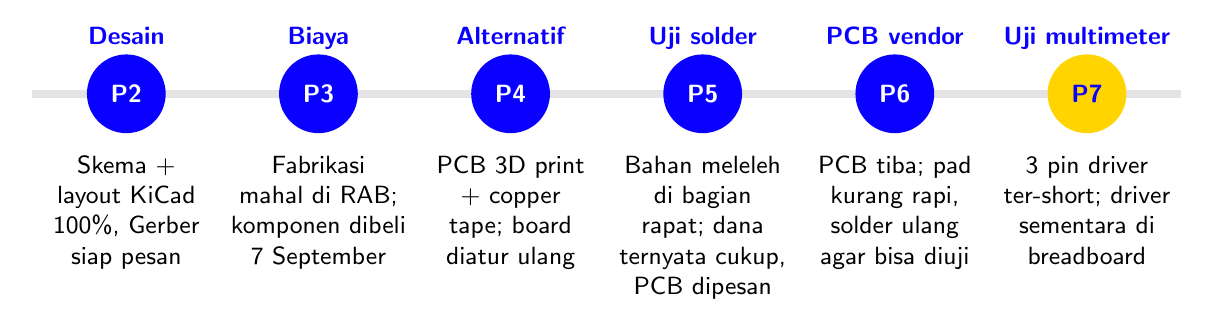
\begin{tikzpicture}
            \draw[track,line width=3pt] (0,0) -- (14.6,0);
            \foreach \x/\colf/\colt/\wk/\ttl/\txt in {
                1.2/rblue/white/2/Desain/{Skema + layout KiCad 100\%, Gerber siap pesan},
                3.64/rblue/white/3/Biaya/{Fabrikasi mahal di RAB; komponen dibeli 7 September},
                6.08/rblue/white/4/Alternatif/{PCB 3D print + copper tape; board diatur ulang},
                8.52/rblue/white/5/Uji solder/{Bahan meleleh di bagian rapat; dana ternyata cukup, PCB dipesan},
                10.96/rblue/white/6/PCB vendor/{PCB tiba; pad kurang rapi, solder ulang agar bisa diuji},
                13.4/ryel/rblue/7/Uji multimeter/{3 pin driver ter-short; driver sementara di breadboard}}{
                \node[circle,fill=\colf,text=\colt,font=\small\bfseries,minimum size=1.0cm,inner sep=0pt] at (\x,0) {P\wk};
                \node[anchor=base,font=\small\bfseries,text=rblue,inner sep=0pt] at (\x,0.62) {\ttl};
                \node[anchor=north,text width=2.3cm,align=center,font=\small,inner sep=0pt] at (\x,-0.78) {\txt};
            }
        \end{tikzpicture}
        \takeaway{Desain kelistrikan lulus pengecekan KiCad (\hl{0 error, 0 unrouted}); short pada 3 pin driver berasal dari \hl{PCB vendor}, bukan komponen driver.}
    \end{frame}

%==================================================================
% [BARU] METODE DAN PARAMETER PENGUJIAN
%==================================================================
    \sect{05}{Pengujian yang telah dilakukan}
    \begin{frame}{Metode dan parameter pengujian}
        \tablestyle
        \renewcommand{\arraystretch}{1.1}
        \begin{tabularx}{\textwidth}{L{3.6cm} Y Y}
    \rowcolor{rblue}\hd{Pengujian}&\hd{Metode}&\hd{Parameter yang diukur}\\
    \rowcolor{white}\textbf{\color{rblue}Layout PCB}&Pengecekan desain di KiCad&Jumlah error dan jalur unrouted\\
    \rowcolor{mist}\textbf{\color{rblue}Mapping di Gazebo}&Menjalankan SLAM di simulasi dunia gedung&Dinding dan ruang terbaca pada peta\\
    \rowcolor{white}\textbf{\color{rblue}Sensor LiDAR}&Membaca data LiDAR di laptop&Data pemindaian terbaca\\
    \rowcolor{mist}\textbf{\color{rblue}Model 3D chassis}&Membuka model di slicer sebelum dicetak&Terbaca slicer tanpa error\\
    \rowcolor{white}\textbf{\color{rblue}Assembly chassis}&Merakit pelat chassis dan motor&Kelengkapan komponen terpasang\\
    \rowcolor{mist}\textbf{\color{rblue}Lokalisasi (simulasi)}&Membandingkan pose robot terhadap peta di simulasi&Presisi posisi (drift)\\
    \rowcolor{white}\textbf{\color{rblue}Elektrikal dan PCB}&Pengukuran dengan multimeter&Short antar pin; fungsi board\\
    \hline
        \end{tabularx}
    \end{frame}

%==================================================================
% 13 - PENGUJIAN
%==================================================================
    \sect{05}{Pengujian yang telah dilakukan}
    \begin{frame}{Tujuh pengujian, empat sudah lulus}
        \tablestyle
        \renewcommand{\arraystretch}{1.0}
        \begin{tabularx}{\textwidth}{L{3.5cm} Y Y L{1.2cm} L{2.2cm}}
    \rowcolor{rblue}\hd{Parameter}&\hd{Target}&\hd{Hasil}&\hd{Pekan}&\hd{Status}\\
    \rowcolor{white}Layout PCB (KiCad)&0 error&Siap cetak&2--3&\lulus\\
    \rowcolor{mist}Mapping di Gazebo&Dinding terbaca&Ruang terbaca&2&\lulus\\
    \rowcolor{white}Sensor LiDAR&Terbaca&Berjalan baik&3--5&\lulus\\
    \rowcolor{mist}Model 3D chassis&Terbaca slicer&Tanpa error&4&\lulus\\
    \rowcolor{white}Assembly chassis&Terpasang semua&Sebagian&5--7&\proses\\
    \rowcolor{mist}Lokalisasi (simulasi)&Posisi presisi&Masih ada drift&2--7&\belum\\
    \rowcolor{white}Elektrikal dan PCB&Berfungsi, tanpa short&Short di 3 pin driver (multimeter)&5--7&\gagal\\
    \hline
        \end{tabularx}
        \takeawayc{Short 3 pin driver berasal dari \hl{PCB vendor}; \hl{drift lokalisasi} juga masih tersisa.}
    \end{frame}

%==================================================================
% 14 - [W7] TARGET PEKAN 7
%==================================================================
    \sect{06}{Hasil sementara}
    \begin{frame}{Target Pekan 7: empat dari lima tercapai}
        \tablestyle
        \renewcommand{\arraystretch}{1.3}
        \begin{tabularx}{\textwidth}{L{0.7cm} L{4.6cm} Y L{2.2cm}}
    \rowcolor{rblue}\hd{No}&\hd{Target}&\hd{Hasil}&\hd{Status}\\
    \rowcolor{white}1&Pembuatan arena maze&Belum jadi: dua anggota sakit dan fokus pekan ini prototype robot&\belum\\
    \rowcolor{mist}2&Finalisasi PCB&Desain final selesai (100\%); PCB vendor diterima dan disolder&\tercapai\\
    \rowcolor{white}3&Fitur dan fungsionalitas frontend app monitoring&Struktur CSS responsif dan 5 menu; app tampil di LCD Raspi&\tercapai\\
    \rowcolor{mist}4&Arsitektur dasar model computer vision&Arsitektur dasar dirancang; script training dibuat&\tercapai\\
    \rowcolor{white}5&Pencarian dataset computer vision&Dataset Obstacle\_detection (train, valid, test) siap&\tercapai\\
    \hline
        \end{tabularx}
    \end{frame}

%==================================================================
% 15 - HASIL SEMENTARA: PROGRES KOMPONEN
%==================================================================
    \sect{06}{Hasil sementara}
    \begin{frame}{Progres proyek per komponen (Pekan 7)}
        \begin{columns}[T]
            \begin{column}{0.64\textwidth}
                \lbar{Bobot dan progres tiap komponen}
                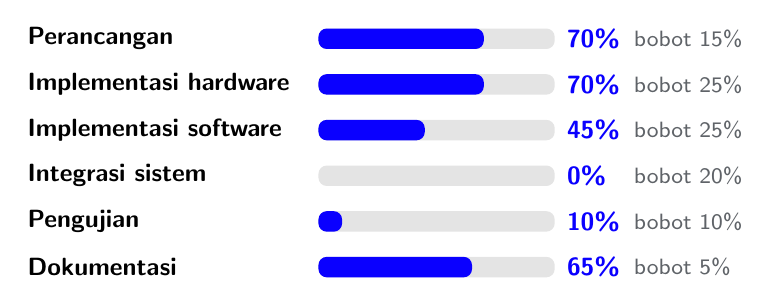
\begin{tikzpicture}
                    \foreach \y/\lbl/\w/\p in {0/{Perancangan}/15/70,1/{Implementasi hardware}/25/70,
                    2/{Implementasi software}/25/45,3/{Integrasi sistem}/20/0,4/{Pengujian}/10/10,5/{Dokumentasi}/5/65}{
                        \node[anchor=west,font=\small\bfseries,inner sep=0pt] at (0,-\y*0.58) {\lbl};
                        \fill[track,rounded corners=3pt] (3.7,-\y*0.58-0.13) rectangle ++(3.0,0.26);
                        \pgfmathsetmacro{\bw}{3.0*\p/100}
                        \ifdim\bw pt>0pt
                        \fill[rblue,rounded corners=3pt] (3.7,-\y*0.58-0.13) rectangle ++(\bw,0.26);
                        \fi
                        \node[anchor=west,font=\small\bfseries,text=rblue,inner sep=0pt] at (6.85,-\y*0.58) {\p\%};
                        \node[anchor=west,font=\footnotesize,text=slate,inner sep=0pt] at (7.7,-\y*0.58) {bobot \w\%};
                    }
                \end{tikzpicture}
            \end{column}
            \begin{column}{0.33\textwidth}
                \lbary{Progres total}
                \centering
                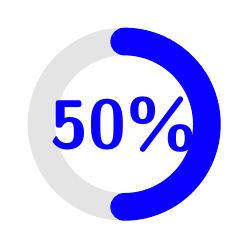
\begin{tikzpicture}
                    \draw[track,line width=10pt] (0,0) circle (1.05);
                    \draw[rblue,line width=10pt,line cap=round] (90:1.05) arc (90:-90:1.05);
                    \node[font=\fontsize{24}{26}\selectfont\bfseries,text=rblue] at (0,0) {50\%};
                \end{tikzpicture}
            \end{column}
        \end{columns}
        \takeaway{Progres total \hl{50\%} (Pekan 6: 45\%); dokumentasi naik ke \hl{65\%}; integrasi sistem masih 0\%.}
    \end{frame}

%==================================================================
% 16 - HASIL PENGUJIAN AWAL
%==================================================================
    \sect{06}{Hasil sementara}
    \begin{frame}[shrink=6]{Hasil pengujian awal}
        \tablestyle
        \renewcommand{\arraystretch}{1.15}
        \begin{tabularx}{\textwidth}{L{3.3cm} Y Y L{1.5cm}}
    \rowcolor{rblue}\hd{Metrik}&\hd{Metode \& alat ukur}&\hd{Hasil}&\hd{Status}\\
    \rowcolor{white}\textbf{\color{rblue}Akurasi dimensi peta}&Bounding box peta SLAM vs GT gedung 9,0$\times$6,0 m&Error 2,46\% \& 1,10\%&\tercapai\\
    \rowcolor{mist}\textbf{\color{rblue}Akurasi okupansi peta (IoU)}&Overlay grid peta SLAM vs peta GT dari \texttt{building\_floor.world}&38,9\% (tol.\ 1 sel: 57,7\%)&\proses\\
    \rowcolor{white}\textbf{\color{rblue}Error posisi dinding}&Offset peta SLAM vs garis dinding GT&mean 2,3 cm; p90 3,3 cm&\tercapai\\
    \rowcolor{mist}\textbf{\color{rblue}Drift odometri/encoder}&Jalan lurus $\approx$5 m, banding jarak GT&error jarak 0,83\%&\tercapai\\
    \rowcolor{white}\textbf{\color{rblue}Drift posisi (loop tertutup)}&Kembali ke titik awal, banding posisi GT&drift akhir 10,2 cm&\proses\\
    \hline
        \end{tabularx}
        \takeawayc{Dimensi peta dan posisi dinding sudah akurat (\hl{2,46\%} \& \hl{2,3 cm}); IoU peta masih perlu ditingkatkan.}
    \end{frame}

%==================================================================
% [BARU] PEMBAGIAN TUGAS ANGGOTA
%==================================================================
    \sect{06}{Hasil sementara}
    \begin{frame}{Pembagian tugas anggota}
        \tablestyle
        \renewcommand{\arraystretch}{1.3}
        \begin{tabularx}{\textwidth}{L{4.2cm} L{3.1cm} Y}
    \rowcolor{rblue}\hd{Nama}&\hd{Peran}&\hd{Tugas utama}\\
    \rowcolor{white}\textbf{Bastian Ramy Ervandi} (Ketua)&Ketua; arena uji&Pembuatan arena robot: limit-test dan maze\\
    \rowcolor{mist}\textbf{Rafsya Ghaizan Athari}&PCB&Desain, revisi, dan perbaikan PCB (KiCad)\\
    \rowcolor{white}\textbf{Muhammad Haidar Al Ghifari}&Robot dan software robot&Assembly chassis, simulasi Gazebo, lokalisasi, navigasi, rosbridge, integrasi LCD ke Raspi\\
    \rowcolor{mist}\textbf{Grace Yunike Margaretha Sitorus}&Monitoring&UI dan frontend dashboard monitoring\\
    \rowcolor{white}\textbf{Muhammad Bryan Farras}&PCB dan computer vision&Solder PCB (Pekan 6); dataset dan script training CV (Pekan 7)\\
    \hline
        \end{tabularx}
    \end{frame}

%==================================================================
% [BARU] STATUS ANGGARAN DAN PENGADAAN
%==================================================================
    \sect{06}{Hasil sementara}
    \begin{frame}{Status anggaran dan pengadaan}
        \tablestyle
        \renewcommand{\arraystretch}{1.0}
        % CATATAN: tambahkan nominal (terpakai / sisa) dari RAB bila diperlukan.
        \begin{tabularx}{\textwidth}{L{3.6cm} Y Y}
    \rowcolor{rblue}\hd{Item}&\hd{Status pengadaan}&\hd{Catatan anggaran}\\
    \rowcolor{white}\textbf{\color{rblue}Komponen utama}&Tersedia: LiDAR, Raspi 4B + Cam, ESP32, MPU, DC motor, LCD&Komponen dibeli 7 September\\
    \rowcolor{mist}\textbf{\color{rblue}PCB}&PCB vendor diterima (Pekan 6); komponen kecil masih dikirim&Fabrikasi internasional mahal di RAB; PCB dipesan setelah dana cukup\\
    \rowcolor{white}\textbf{\color{rblue}Chassis}&Part 3D print tersedia dan terakit sementara&Dibuat dengan 3D print\\
    \rowcolor{mist}\textbf{\color{rblue}Arena uji}&Limit-test jadi; maze belum jadi&Budget kurang: bahan daur ulang, ukuran diperkecil\\
    \hline
        \end{tabularx}
        \takeawayc{Dana mencukupi untuk PCB vendor; arena memakai \hl{bahan daur ulang} karena budget terbatas.}
    \end{frame}

%==================================================================
% 17 - KENDALA
%==================================================================
    \sect{07}{Kendala \& risiko}
    \begin{frame}{Lima kendala utama dan penanganannya}
        \tablestyle
        \renewcommand{\arraystretch}{1.2}
        \begin{tabularx}{\textwidth}{Y Y L{2.1cm}}
    \rowcolor{rblue}\hd{Kendala dan dampak}&\hd{Penanganan}&\hd{Status}\\
    \rowcolor{white}\textbf{PCB 3D print meleleh saat disolder.} Desain compact merusak jalur.&Desain ulang; PCB cetak vendor setelah dana dicek ulang dan cukup.&\teratasi\\
    \rowcolor{mist}\textbf{Short pada 3 pin driver PCB vendor (pin bridging).} Error pada motor driver, prototype tertunda.&Driver disubstitusi dengan breadboard, atau dilakukan pemotongan pada PCB.&\proses\\
    \rowcolor{white}\textbf{Budget arena tidak cukup.} Bahan terbatas.&Bahan daur ulang (kardus, kertas, koran); ukuran arena diperkecil.&\teratasi\\
    \rowcolor{mist}\textbf{Arena maze belum jadi.} Dua anggota sakit; fokus pekan ini prototype robot.&Dijadwalkan ulang ke Pekan 8; arena limit-test sudah tersedia.&\proses\\
    \rowcolor{white}\textbf{Drift lokalisasi di simulasi.} Pose robot di peta kurang presisi.&Evaluasi sistem lokalisasi dan navigasi (Haidar); body robot di simulasi diperbaiki.&\belum\\
    \hline
        \end{tabularx}
    \end{frame}

%==================================================================
% [BARU] RISIKO PENYELESAIAN PROYEK
%==================================================================
    \sect{07}{Kendala \& risiko}
    \begin{frame}{Risiko penyelesaian proyek}
        \tablestyle
        \renewcommand{\arraystretch}{1.25}
        \begin{tabularx}{\textwidth}{Y Y Y L{1.9cm}}
    \rowcolor{rblue}\hd{Risiko}&\hd{Dampak}&\hd{Mitigasi}&\hd{Tingkat}\\
    \rowcolor{white}\textbf{Short pada PCB vendor; driver di breadboard}&Sinyal tidak andal; prototype tertunda&Perbaiki PCB; uji kelistrikan ketat&\tinggi\\
    \rowcolor{mist}\textbf{Integrasi sistem masih 0\%}&Waktu uji menjelang akhir semester sempit&Hardware dulu; siapkan data ROS 2&\tinggi\\
    \rowcolor{white}\textbf{Kapasitas tim turun (anggota sakit)}&Arena maze dan jadwal tertunda&Jadwal ulang; arena limit-test tersedia&\sedang\\
    \rowcolor{mist}\textbf{Drift lokalisasi}&Pose robot kurang presisi&Evaluasi lokalisasi dan navigasi&\sedang\\
    \rowcolor{white}\textbf{Training CV tertunda}&Model CV belum siap saat integrasi&Training CV dijadwalkan 23 Oktober&\sedang\\
    \hline
        \end{tabularx}
    \end{frame}

%==================================================================
% 20 - RENCANA PEKAN KE-8
%==================================================================
    \sect{08}{Rencana hingga akhir semester}
    \begin{frame}{Rencana kerja pekan ke-8}
        \tablestyle
        \renewcommand{\arraystretch}{1.5}
        \begin{tabularx}{\textwidth}{L{2.0cm} Y L{4.0cm}}
    \rowcolor{rblue}\hd{PIC}&\hd{Kegiatan}&\hd{Target selesai}\\
    \rowcolor{white}\textbf{\color{rblue}Bastian}&Menyelesaikan arena 100\%, termasuk versi maze&Jumat, 16 Oktober 2026\\
    \rowcolor{mist}\textbf{\color{rblue}Rafsya}&Pengimprovan PCB&Jumat, 16 Oktober 2026\\
    \rowcolor{white}\textbf{\color{rblue}Haidar}&Evaluasi sistem lokalisasi, navigasi, rosbridge, dan assembly robot&Jumat, 16 Oktober 2026\\
    \rowcolor{mist}\textbf{\color{rblue}Grace}&Pengembangan lanjutan App Monitoring Dashboard dan persiapan integrasi data simulasi ROS 2&Jumat, 16 Oktober 2026\\
    \rowcolor{white}\textbf{\color{rblue}Bryan}&Training CV&23 Oktober 2026\\
    \hline
        \end{tabularx}
    \end{frame}

%==================================================================
% 21 - ROADMAP
%==================================================================
    \sect{08}{Rencana hingga akhir semester}
    \begin{frame}{Empat fase menuju akhir semester}
        \leavevmode{\footnotesize\itshape\color{slate}Usulan jadwal; sesuaikan dengan kalender Desain Proyek 2.}\par\vspace{3pt}
        \begin{columns}[T]
            \begin{column}{0.235\textwidth}
                \begin{phase}{4.45cm}{Pekan 7--8}
                    \small\raggedright\textbf{Hardware 100\%}\\[3pt]
                    \textbullet~PCB selesai dan diuji\\\textbullet~Robot terassemble\\\textbullet~Arena maze selesai
                \end{phase}
            \end{column}
            \begin{column}{0.235\textwidth}
                \begin{phase}{4.45cm}{Pekan 8--9}
                    \small\raggedright\textbf{Software di robot}\\[3pt]
                    \textbullet~SLAM di robot nyata\\\textbullet~Perbaikan drift\\\textbullet~Navigasi + obstacle avoidance\\\textbullet~Training model CV
                \end{phase}
            \end{column}
            \begin{column}{0.235\textwidth}
                \begin{phase}{4.45cm}{Pekan 9--11}
                    \small\raggedright\textbf{Integrasi dan uji}\\[3pt]
                    \textbullet~Robot ke dashboard via rosbridge\\\textbullet~Computer vision terpasang\\\textbullet~Uji limit-test dan maze
                \end{phase}
            \end{column}
            \begin{column}{0.235\textwidth}
                \begin{phase}{4.45cm}{Pekan 12+}
                    \small\raggedright\textbf{Finalisasi}\\[3pt]
                    \textbullet~Kalibrasi akhir\\\textbullet~Dokumentasi dan laporan\\\textbullet~Persiapan demo akhir
                \end{phase}
            \end{column}
        \end{columns}
        \par\vspace{6pt}\begin{dpanel}\small\textbf{\color{rblue}Target akhir semester:} hardware, software, integrasi, pengujian, dan dokumentasi mencapai \hl{100\%}.\end{dpanel}
    \end{frame}

%==================================================================
% 22 - RINGKASAN
%==================================================================
    \sect{08}{}
    \begin{frame}{\large Prototype terus berjalan, integrasi jadi fokus berikutnya}
        \begin{columns}[T]
            \begin{column}{0.315\textwidth}
                \lbar{Sudah dicapai}
                \begin{dpanel}[height=5.4cm]
                    \begin{itemize}\setlength{\itemsep}{4pt}
                        \item Desain PCB selesai; PCB vendor disolder
                        \item Chassis terakit, motor terpasang
                        \item Mapping dan lokalisasi di Gazebo
                        \item App monitoring tampil di LCD Raspi
                        \item Dataset dan script training CV siap
                    \end{itemize}
                \end{dpanel}
            \end{column}
            \begin{column}{0.315\textwidth}
                \lbary{Tantangan}
                \begin{dpanel}[height=5.4cm]
                    \begin{itemize}\setlength{\itemsep}{4pt}
                        \item Short 3 pin driver pada PCB vendor
                        \item Arena maze belum jadi
                        \item Drift lokalisasi
                        \item Integrasi sistem masih 0\%
                    \end{itemize}
                \end{dpanel}
            \end{column}
            \begin{column}{0.315\textwidth}
                \lbar{Fokus berikutnya}
                \begin{dpanel}[height=5.4cm]
                    \begin{itemize}\setlength{\itemsep}{4pt}
                        \item Hardware 100\%
                        \item Arena maze selesai
                        \item Training model CV
                        \item Integrasi robot, dashboard, dan CV
                        \item Uji di arena maze
                    \end{itemize}
                \end{dpanel}
            \end{column}
        \end{columns}
    \end{frame}

%==================================================================
% 23 - PENUTUP
%==================================================================
{
    \setbeamercolor{background canvas}{bg=rblue}
    \setbeamertemplate{footline}{}
    \begin{frame}[plain]
        \begin{tikzpicture}[remember picture,overlay]
            \zigzag
            \logoblock
            \node[text width=14cm,align=center,inner sep=0pt] at ($(current page.center)+(0,0.5)$) {%
                    {\color{ryel}\bfseries\fontsize{40}{44}\selectfont Terima\hspace{0.3em}Kasih}\\[10pt]
                {\color{white}\itshape\large Tanya jawab}\\[14pt]
                {\color{white}\small Autonomous Rover for Guidance Evacuation Routing via SLAM}\\[6pt] % Ditambah line break di sini
                {\color{white}\small Video demo: https://drive.google.com/file/d/1oK\_xC54mHAM0a7nOcS5rIWUxdmSL7mFg/view?usp=drivesdk}}; % Perhatikan penggunaan \_
            \fill[mist,rounded corners=0.4cm]
            ($(current page.south)+(-4.8,-0.6)$) rectangle ($(current page.south)+(4.8,0.7)$);
            \node[font=\footnotesize,text=ink,inner sep=0pt] at ($(current page.south)+(0,0.22)$)
                {Desain Proyek 2 \textperiodcentered{} Kelompok 9 \textperiodcentered{} \presdate};
        \end{tikzpicture}
    \end{frame}
}

\end{document}